
\section{Narvis: System Design and Implementation}
\subsection{An overview}

Narvis aims to offer an efficient, expressive and friendly authoring tool for the experts in data visualization, help them create a slide show for the purpose of introducing an advanced visualization design to general audience.  Thus, it has two kinds of users: editors, the data visualization experts who use Narvis to create an explanation slideshow, and audiences, the general audience who watch the slideshow created by ediors.The working flow of Narvis can be described as three phase: Automatic Analysis Phase, Human Editing Phase, Viewing Phase. 

In Automatic Analysis Phase, the system automatically extracta the graphical elements in the input visualization with an edge-detection-based algorithm. These graphic elements then be classified based on their visual appearance, such as the area, color, the number of corners. Input text descriptions are also classified based on a basic keyword detection and sentence classification approach. 

In Human Editing Phase, editors will be involved to modify the output from the Automatic Analysis Phase. Narvis offers templates and pre-defined animation to better support them to craft a explanation slideshow. 
 
In Reviewing Phase, reviews can assess the slide show generated in Human Editing Phase. Their feedback, more specifically, their click activity and comments, will be recorded and send to the Human Editing Phase, helping improve the quality of the slide show. 

\begin{figure}
 \centering % avoid the use of \begin{center}...\end{center} and use \centering instead (more compact)
 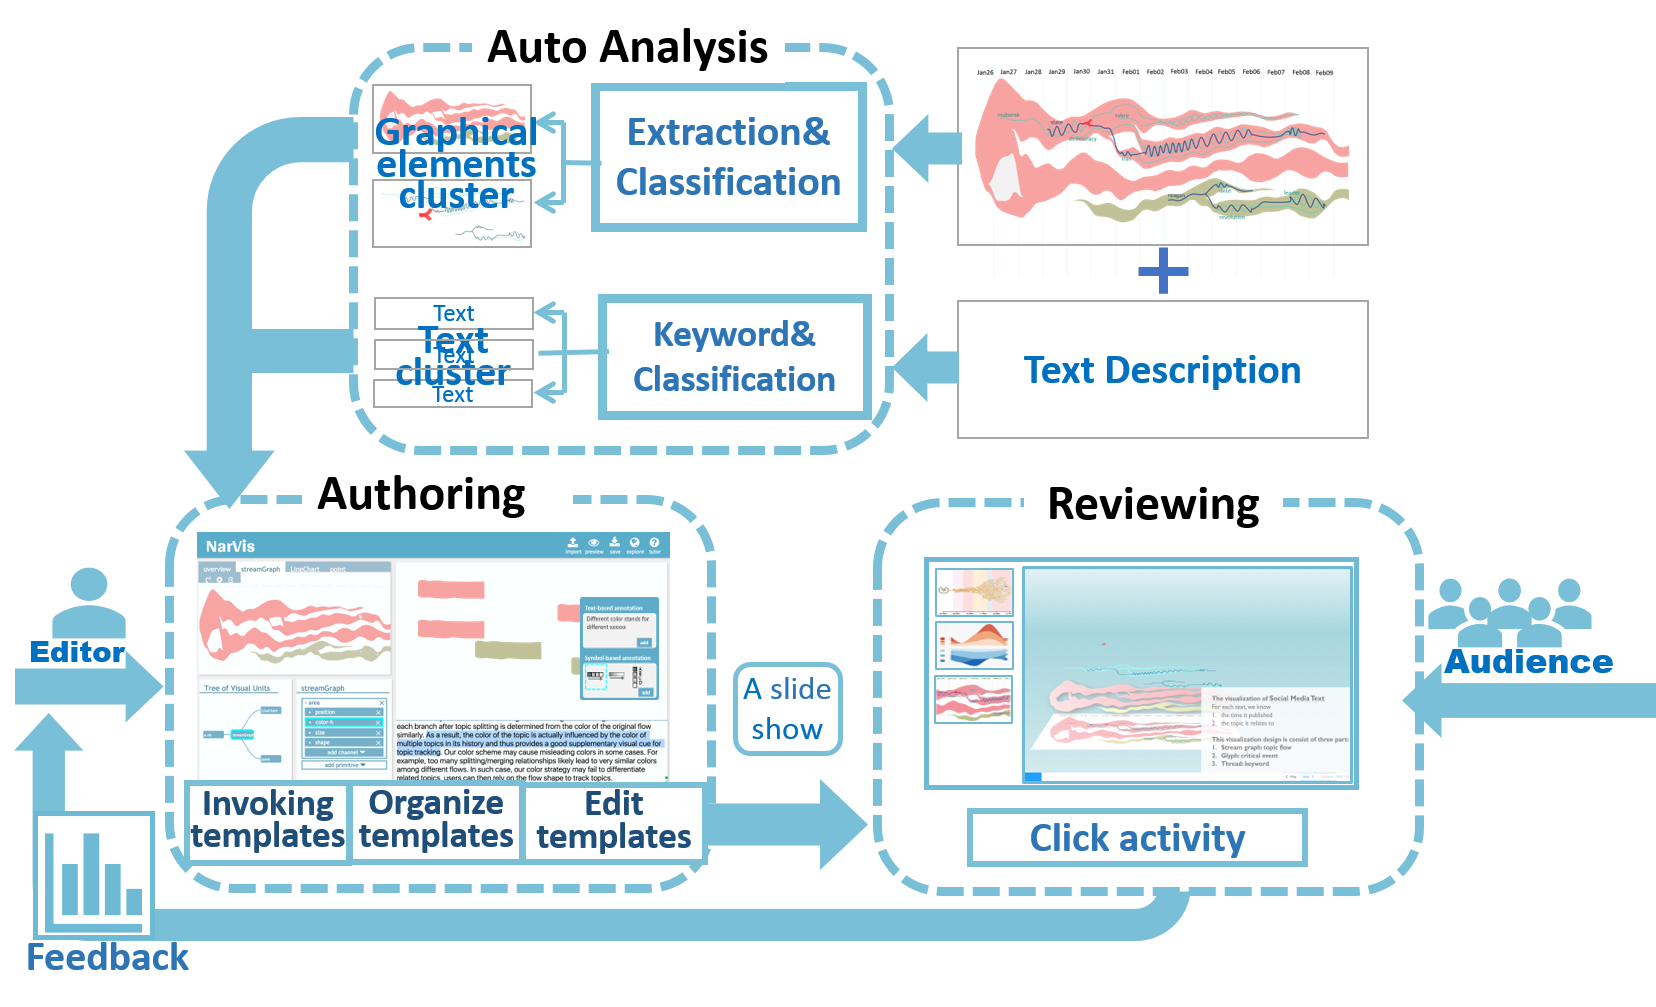
\includegraphics[width=\columnwidth]{overview}
 \caption{The system overview}
 \label{fig:overview}
\end{figure}

\subsection{Design consideration}
We should take editors and audiences alike into consideration for the design of Narvis. In other words, the design tasks should focus on two aspect: offering good authoring experience and improving generated slideshow. 
Hence, we settle on six design considerations(DCs) for this authoring tool. Our premise is that the editor is familiar with a visualization design but unclear how to educate his audiences in an efficient way. Since the background of the audiences cannot be guaranteed, we assume they all have no prior knowledge in data visualization. 

\textbf{DC1. Clear structure and organized narrative sequence.}

The complicated relationship, spatial and logical alike,  between different graphic elements is one of the biggest barriers that impedes a smooth communication of visual encoding scheme. By encouraging users to refine the clusters of graphic elements, to figure out relationship between visual units by editing a unit tree, and to modify the narrative templates we offered, we aim at motivating users to sort out the structure of a visualization, which will then result in a better-organized narrative sequence. 

\textbf{DC2. Control the density of information flow.} 

To avoid information overload, we propose to extract the information distributed spatially in a  figure and reorganize them in a temporal order. The amount of information revealing at a time can be controlled by offering narrative templates for different visual units. 

\textbf{DC3. Emphasis on efficiency}
There are many presentation tools, such as Power Point\footnote{https://office.live.com/start/PowerPoint.aspx}and KeyNote\footnote{http://www.apple.com/keynote/} that can be used for introducing a data visualization. But it can be time-consuming and tedious to use them for introducing a complex visualization, which has lots of graphical elements and various visual grammar.

For example, animations are extensively used to engage audiences and guide their attention to crucial information in narrative data visualization.\cite{amini_authoring_2017, amini_understanding_2015} But editting animation manually can be annoying. A high efficiency construction can be achieved by composing components. \cite{bostock_protovis:_2009, huron_constructive_2014} 
%Instead of letting the users edit manually on a case-by-case basis, we offer several animation sequences by considering the operations one might apply when explaining a visualization.

\textbf{DC4. Avoid unconscious ignorance}

Experts in data visualization, prone to treat some visual encodings as evident, might unconsciously ignore some crucial information when introducing a visualization to ordinal people. However, for these with no prior knowledge about data visualization, the lack of such information can totally confuse them. By restricting users' operation on combining and editing the offered explanation templates, which has a full coverage of all the possible encodings, we aim to eliminate such unconscious ignorances.   \par
\textbf{DC5. Emphasis on conveying intuitive concepts.} The audience of the generated narrative explanations are ordinal people, and they usually have no interests in understanding the algorithm employed in a visualization design. For example, the comprehension that a transition line indicates public attention shift from one topic to another is enough for them. Explicating how to quantify public attention shift only bores the audience, even scares them away. Although such algorithm might be crucial for the achievement of a visualization design, by providing simplified sentence pattern for annotation adding, we skip such parts in purpose.

\textbf{DC6. Support feedback.} Having access to the audience's feedback is crucial for the editors to improve  the quality of their introduction, making it more understandable and attractive.  We implement a click collector which will automatically record click activity when audience view the explanation in our system. The click stream data can reveal information about viewing order, for example, the audience might skip one slide or go back to revisit another, the time spent on each slide, the degree of understanding at each part.The audience can also write down their comments while reviewing such an introduction slide show. Editor can adjust the narrative sequence as well the level of details based on these feedbacks. 
\subsection{Phase1: Auto Analysis}\par
The auto analysis has two parts: one for input image and one for input text. Note that the textual input is not necessary but it provides hints when editors add annotations manually in the Human Editing Phase.
 \subsubsection{Analysis of input image}
The auto analysis of input image has three main steps. It first detects all primitives that it finds in the given image and also detects any labels that are present in the visualization. It will then cluster objects that are spacially linked and extract non-target objects. Finally, it will fill in any empty spaces left inside objects from extraction with the appropriate color so as to show the target object in its entirety.

The first step, object detection, is done by iterating through all the pixels on the bitmap. At every iteration, we first check to see if this pixel has already been tagged as part of an object. If not, we know that this pixel forms a part of a new object.We explore the colors of the neighboring pixels, where the neighbors are chosen such that the distance between the current pixel and a potential neighbor is less than 3. If the difference in color between a neighbor pixel and the current pixel is less than a threshhold, the neighboring pixel is tagged as part of the same object. Once all neighbors have been classified as either part of the same object or not, we choose another pixel that was classified as part of the same object and apply this algorithm again. This is a modified BFS algorithm and allows us to identify all unique ojects in the given visualization.

Once all the objects have been detected, we have to extract a target object. To extract an object means to only select the pixels that are classified as part of this object, so we should remove all objects that are not part of this object and we should extract objects that are inside our target object.It is trivial to set all pixels that are not within or part of our object to have color white. For objects that are inside our target object, i.e. those objects that are clustered with out target object, we will first detect that object then programmatically change its pixels to white.

Once we have completed extraction, we have the issue of these white spaces. The reason this is an issue is because an extracted object might have been dividing two objects, and so when it is extracted, we lose the boundary between our target object and another object, which can cause confusion as to whether that white space should be colored in or not. To solve this boundary problem, we create a queue of the white spaces, with each data point giving the starting and ending point of that space. We then look at the intervals between enclosed white spaced objects, if that interval is above a threshhold, we take that white space to not be part of our object. If it is below our threshhold, then we enclose the white space with the target objects color, creating a boundary for it. The main difference is that for objects not within our target object, we do not create a boundary, whereas objects within our target object are enclosed with the target objects color.\par
\subsubsection{Analysis of input textual description}
For the input textual description, we offer a basic text detection and classification algorithm, which uses a dictionary of terms that are highly correlated with certain channels. E.g. the word "length" is highly correlated with the size channel. To do the text detection, we first classify each sentence depending on whether it contains any of the key words in our dictionary. If it contains a key word for one of the channels, the sentence is tagged as being a description of that channels visualization. Once we have tagged all the sentences, whenever a channel is selected, we show the entire text that was inputted and highlight the text that has been tagged as descriptive of that channels visualization.

The algorithm we proposed is a compromise between efficiency and performance. At this time point, it is limited for image with high quality and clear edges, but its performance can be improved by applying a more advanced algorithm, such as the method based on patch detection and clustering mentioned in Revison\cite{savva_revision:_2011}.

\subsection{Phase2: Human Editing}
\subsubsection{The interface for editing}
The interface of editing mode is composed of the following panels.We arrange the position of these panels and their content to better match the observed authoring work flow: refine clusters-> bind with templates ->organize the structure of visual units->modify templates ->add annotation. 

\textbf{\textit{FigSource}: extracting and organizing graphic elements}\par
FigSource is a tabbed panel where the extracted graphical elements are associated with different tabs based on the pre-cluster results. The user add, delete, modify the graphical elements associated with each tab, making sure that 1) All the graphical elements of the same visual unit is with one tab 2) every graphical element belongs to one and only one tab. For each tab, which actually equals to a visual unit now, the user call a template from our library with a drop-down list. 

The templates, using the color, shape and position of the input graphical elements, generate a sequence of slides that tends introduce a certain visual unit.

\textbf{\textit{Unit tree}: clarify the structure of a visualization}
\textit{Unit tree} panel tends to motivate the users to figure out the relationships between different visual units througn interacting.  
In the \textit{Unit Tree} panel, all visual units are shown as tree nodes.
With Interactions as simple as dragging and dropping, the users organized and display the structure of the visual units in the panel, like what we have discussed in section 3.3. To help people better identify the relationship between visual units, which might be a new concept for them, we include a tutorial here. Even though learning the relationship between visual units requires extra effort and time, we believe it is worthwhile since it can give people a better understanding about the structure of a visualization. Based on the tree diagram, Narvis will refresh the narrative sequence of visual units. 

 \textbf{\textit{ In-unit \& Editor panel}: personalized modification}
 
 Narvis provides templates to achieve high efficiency, but it also allow the users high flexibity to modify these temples, thus guaranteeing the expressiveness of this system. 
 
For each visual units, narvis enumerates all possible encodings and recommends a narrative sequence based on the metrics we mentioned in section 3.1.4. In the \textit{In-unit} panel, editors can edit a template by selecting a node on the \textit{Unit tree} panel. They are allowed to delete channels which are not employed in their visualization design,  and adjust the narrative sequence of explaining based on their cases. 
 
In the editor panel, users get further to access the \textit{grammar} of each visual primitives, add annotation to describe it, refine the attention cue we embedded in a template. 

\subsubsection{A library of templates}
We propose a library of templates for the narrative explanation of a visualization. A templates is a set of slides that tends to introduce a visual unit, which can be descibed as an orthogonal combination of a visual primitive and a construction rule, as mentioned in section 3.1.1. Since advanced visualization design is the assembly of miscellaneous visual units, we conjecture such templates can achieve a high level of efficiency for the explanation of a viusalization. Meanwhile, allowing users a high flexible, friendly interface to edit offered templates, Narvis maintains a considerable level of expressiveness and accessibility. 

\textbf{Templates design}

With a visual unit, more specifically, a set of graphic elements, as an input, these templates are aimed to provide 1) a well-considered narrative sequence for visual encoding explanation; 2) Embedded attention cues and animated transitions that orientate visual attention  when people view this slide show; 3) Formatted sentence for annotations that will be gradually disclosed in the slide show. 

\textbf{Types of Templates}

As described in section3.1, a visual unit is the orthogonal combination of visual primitives and assembly rules.   

We now describe the initial set of graphical primitives provided by Narvis. Narvis is extensible, new templates can be introduced by web programmers as well as by end users with no programming skills. At the same time, it is desirable to condense the set of supported templates into several types, so as to avoid overwhelming users with a cornucopia of confusing options.\par
theme river, \par
node link, \par
sankey diagram, \par
radial diagram,\par
scatter plot,\par 
chart,\par
donut chart\par
\subsubsection{Utility}
We demonstrate the utility of this library from the following aspects:
\textbf{Efficiency}\par
\textbf{Expressiveness}\par
\textbf{Accessibility}\par
To broaden the coverage of Narvis, we enable users high flexibility to edit the templates we provide. For example, for the triangle scatter plot in Opinion Seer\cite{wu_opinionseer:_2010}, which is a novel visualization design, we just need to edit the explanation template for ordinal scatter plot in our library, changing the position channel from "x-y position" to "force-direct region".  
Through a high flexible interaction, the coverage of our library can reach up to xxx  without extra programming work. 
% \textbf{full coverage}\par refers to that the templates need no change to craft a sense-making narrative explanation. 
% \textbf{minor adjustment needed} refers to editing the current templates 
% \textbf{major adjustment needed} means the implementation of new templates is needed. 

\textbf{Animation embedded in templates }
Narvis mainpulates transition to reveal the encodings of a visual primitive gradually, thus reducing the study burden of audiences. Thus, maintaing object constancy is attached with great importance in our design. 
We offer the following animated transitions to support easy creation of animations in a narrative data visualization environment.\par 
\textbf{Morphing:} morphing is widely applied to demonstrate the changing of size and shape of a graphic element. Thus, it can be an effective method to attract audiences' attention when explaining the encoding of these two visual channels. \par
\textbf{Moving:} such kind of animated transition change the position of graphic elements, making it intrinsically suitable for revealing the encoding of position. \par 
\textbf{Blur:} A common strategy applied in "focus + context" technique to discriminate focus from its context. In Narvis, we blur all the graphic elements of a visual unit when we finish the explanation of this visual unit and move to another one. \par
\textbf{Flicker:} as with blur, flicker is also used in "focus + context" technique. Unlike blur, which  erase contextual details, flicker achieve minimal deformation of context but at the cost of introducing annoyance. \par
\textbf{Zoom-in/out:} We offer the option of zoom-in/out effect for emphasizing graphic elements whose size are small. However, giving high priority to the sense of overview, we do not recommend such animated transition in our explanation templates.  \par
\textbf{Annotation:} Progressively disclosing annotations while highlighting the related graphic elements can facilitate perceptional progress by enhancing the connection between data and graphic elements.\cite{bryan_temporal_2016}  \par
\textbf{Information repetition:} Slides are automatically inserted at certain points to conduct information repetition in the form of questions or summaries. \par 
The frequency of information repetition is determined by the mode users choose. \par
\subsection{Phase3: Viewing}
\subsubsection{The interface for audience}
The interface of audience is composed of two panels.

\textbf{\textit{Gallery:}the collection of generated slide show}
 
Gallery exhibit all the slide show produced by editors and saved in Narvis. Every slide show is presented by a image, the visualization it tends to explain. By clicking on the image, users can watch this slide show in the \textit{Screen} panel. 

\textbf{\textit{Screen:}  review and comment}
Every slide show displayed in \textit{Gallery}is a series of slides, each of which is responsible for the delivery of one simple encoding information, for example, the horizontal position indicates time. In the \textit{Screen} panel, users click buttons to move forward or backward to view these slides. 
\subsubsection{Generated Report}

\subsection{A working scenario}
Here, we demonstrate the utility of Narvis through the creation of a narrative explanation of a visualization design that published in TVCG (http://ieeexplore.ieee.org/stamp/stamp.jsp?arnumber=5613449). 
\subsubsection{Motivation}Jessica, a expert in data visualization, realizes the promising prospect of implementing this visualization design in an on-line review service website like Yelp. (pg student to classmates? prof to a journalist? prof with collaborators from other fields?  )\par
However, she has to present this design in a general meeting to get the financial support. She is familiar with this visualization design, yet not sure whether her audiences, with little knowledge about data visualization, can quickly learn this visualization design from her introduction. Without clear awareness of the visual encodings, audience can hardly identify the interesting patterns this visualization reveals and realize its utility.  \par
A traditional way is to add highlights and annotations in the original visualization. But Jessica worries about the effectiveness of information delivery. \par
She considers about applying "focus + context" techniques,  but it will introduce some complicated operations for her, who has no experience in image editing. \par
Moreover, with the large number of visual encodings existing, she fails to determine an optimized order for explaining them. Even though she has many years of experience in data visualization, she never think about this issue before. \par
She then turns to Narvis for help. 
\subsubsection{Editing Procedure}
She first imports her visualization design, in the form of a PNG file, and the corresponding text description, which she directly copy from the paper, into the system. After a few seconds, the system will automatically detect graphics elements with a edge detection algorithm and cluster them based on their features. The algorithm cannot be perfect. For example, it puts geo ring and calendar ring in the same cluster based on their similar appearance. \par
Jessica then refines the automatic cluster results, making sure every graphic elements in one visual unit is put in one cluster \textbf{figure xxx}. After that, she chooses narrative templates for each cluster, thus obtain 4 units in the \textbf{unit tree} panel. The triangle scatter plot is a novel design that the library has no narrative template matching it. Jessica then chooses the template for regular scatter plot, whose only difference to triangle plot is the encoding of position. \par
Now, Jessica has four visual units in the unit tree panel showing in the form as tree nodes. By an easy dragging interaction, April organize the structure of the tree based on the relationships between units, as we discussed in section 3.3.\textbf{fig xxxx}\par
Then Jessica edits the narrative templates based on her design. In the templates, we enumerate all the possible visual encodings. April goes through all four templates in the "in-unit", delete the visual channels that has no encodings. \par
At this time point, a slide-show has already generated with the defaulted animated transitions. But Jessica can further improve its quality by adding annotations into animations, strengthening the binding between data and graphic elements. \par
When adding annotation to a certain channel, the related text will highlight in the text area, aiming to offer a better user experience. \par  
\subsubsection{Collect feedback}

Before the general meeting, Jessica ask several friends, who have no experience in data visualization, to review her introduction slide show. Jessica can access to their feedback from their click activity, which is automatically recorded by Narvis. These click stream data, revealing information such as, "which slide they skip", "which slide they go back to revisit", and "which slide they spend abnormally long time on", provides cues for Jessica to strengthen the understandability as well as attractiveness of her introduction slide show.  